\documentclass[a4paper,10pt]{article}
\usepackage[margin=1cm]{geometry}
\usepackage{multicol}
\usepackage{fancyhdr}
\usepackage{listings}
\usepackage{graphicx}

% Metadata
\title{Trabalho 2 - Coinnect - Modelo Cliente/Servidor (RPC/RMI)}
\author{Bruno Carlan \\ Gabriela Dellamora \\ Leonardo Ripes \\ Luize Iensse}
\date{\today}

% Header
\pagestyle{fancy}
\fancyhf{}
\fancyhead[L]{Pontifícia Universidade Católica do Rio Grande do Sul}
\fancyhead[R]{Fundamentos de Processamento Paralelo e Distribuído}
\fancyfoot[C]{\thepage}

\begin{document}

\maketitle

\begin{abstract}
Este documento apresenta o trabalho desenvolvido para a disciplina de Fundamentos de Processamento Paralelo e Distribuído. O projeto implementa um sistema distribuído baseado no modelo Cliente/Servidor, utilizando RPC/RMI para simular operações bancárias.

\end{abstract}

\begin{multicols}{2}

\section{Introdução}

Este relatório explora a implementação de um sistema bancário em Go, com uma arquitetura cliente-servidor baseada em chamadas de procedimento remoto (Remote Procedure Call, ou RPC). O sistema foi modularizado em três pacotes principais: ATM (Caixa Automático), que permite aos clientes realizarem transações como saques, depósitos e consultas de saldo; BankManager (Administração), que centraliza o gerenciamento de contas e operações bancárias no servidor; e BankBranch (Agência), que atua como intermediário entre o cliente e o servidor. Essa estrutura modular facilita a manutenção e ampliação do sistema, promovendo flexibilidade e escalabilidade na arquitetura. Neste relatório, cada módulo será abordado detalhadamente, com foco nas funcionalidades de cada camada e nos mecanismos de controle de concorrência e idempotência, essenciais para a segurança e eficiência das operações bancárias.

\section{Arquitetura do Sistema}

O sistema foi projetado com o modelo cliente-servidor utilizando RPC para possibilitar que clientes remotos possam realizar operações bancárias como saques, depósitos e consultas de saldo. Cada operação é uma função no servidor (BankManager), que é acionada remotamente pelo cliente via RPC. O módulo ATM, atuando como cliente, envia as solicitações ao módulo BankBranch (Agência), responsável por gerenciar as comunicações e transmitir as operações ao servidor. Esse modelo modular, além de otimizar a organização do código, facilita a manutenção e escalabilidade do sistema, uma vez que cada componente pode ser aprimorado de forma independente.

Ao utilizar RPC, o sistema permite que operações sejam solicitadas de qualquer lugar com conexão ao servidor, mantendo uma resposta rápida e sem a necessidade de configuração avançada pelo cliente. O uso de RPC proporciona uma experiência mais ágil para o usuário, dado que o cliente envia comandos diretos para o servidor, minimizando latências e simplificando a comunicação entre os componentes.

\subsection{Processo Administração}

O processo Administração, implementado na camada BankManager, é responsável pela gestão das contas bancárias e pela execução de operações críticas, como a abertura e fechamento de contas, saques e depósitos. Este processo é fundamental para assegurar a integridade dos dados do sistema e garantir que as operações sejam executadas de forma segura em um ambiente concorrente.

\subsection{Processo Agência}

O processo Agência, encapsulado no pacote BankBranch, fornece uma interface para a interação do cliente com as funcionalidades do banco. Ele permite que os usuários abram novas contas, realizem saques, depósitos e consultem saldos. As chamadas feitas pelo cliente ao servidor são mediadas por funções RPC que invocam operações específicas do servidor. Cada chamada é tratada de forma assíncrona, garantindo que a interface do usuário permaneça responsiva enquanto as operações estão em andamento.

\subsection{Processo Caixa Automático}

O processo Caixa Automático, encapsulado no pacote ATM, oferece aos clientes uma interface direta para realizar transações bancárias, como saques, depósitos e consultas de saldo. Este sistema permite que os usuários interajam com suas contas de maneira conveniente e eficiente, sem a necessidade de atendimento presencial.

\section{Controle de Concorrência}

O controle de concorrência foi implementado para garantir a segurança das operações de contas quando múltiplos clientes acessam simultaneamente o sistema. O BankManager utiliza mutexes para proteger as operações críticas, como criação de contas e movimentação de saldo, assegurando que as transações ocorrem de forma atômica e consistente.

\subsection{Implementação}

Em Go, mutexes foram utilizados para bloquear temporariamente a estrutura de dados enquanto uma operação estava em andamento. Cada operação que envolvia uma modificação no saldo ou criação de contas era protegida por uma exclusão mútua (mutex lock), garantindo que apenas uma operação de escrita ocorresse por vez. Essa implementação evita problemas como a criação de contas duplicadas ou a inconsistência nos saldos devido a condições de corrida.

\subsection{Testes de Concorrência}

Para testar o controle de concorrência, múltiplas instâncias de clientes foram simuladas acessando e alterando simultaneamente o saldo de uma conta específica. Os testes verificaram que nenhuma condição de corrida ocorria, assegurando que as operações críticas eram concluídas de forma segura e coerente. Além disso, testes adicionais foram realizados com operações simultâneas em contas diferentes para avaliar o desempenho e garantir que o sistema mantinha a integridade dos dados em ambientes com alto volume de requisições.

\section{Controle de Idempotência}

Para garantir que operações idênticas produzissem os mesmos resultados, mesmo em casos de falhas de rede ou duplicação de solicitações, foi implementado o controle de idempotência no BankManager. Este controle assegura que operações repetidas, como saques ou encerramento de contas, não causem efeitos indesejados no sistema.

\subsection{Implementação}

Cada operação RPC possui um identificador único associado à solicitação inicial. Quando uma requisição é recebida pelo servidor, ele verifica se já processou aquele identificador, retornando o resultado anterior se necessário. Esse método foi aplicado em operações de saque e encerramento de conta, garantindo que uma mesma solicitação não afete o sistema repetidas vezes, prevenindo, por exemplo, saques múltiplos do mesmo valor ou fechamento duplicado de uma conta.

\subsection{Testes de Idempotência}

O controle de idempotência foi testado simulando falhas e repetição de operações. Por exemplo, em um teste de saque duplicado, duas requisições idênticas foram enviadas para sacar o mesmo valor de uma conta. O sistema reconheceu a segunda solicitação como repetida e retornou o mesmo resultado da primeira operação, sem duplicar o saque. Esse tipo de teste foi aplicado em diversas operações para garantir que as ações idempotentes funcionavam conforme esperado, e que o sistema mantinha sua integridade mesmo sob falhas.
Este controle de idempotência é particularmente eficaz contra falhas de rede, onde operações podem ser reenviadas inadvertidamente por tentativas de reconexão do cliente. A reutilização do resultado da operação anterior evita inconsistências no banco de dados.
Durante os testes de idempotência, foram realizadas simulações de falhas de rede onde operações idênticas foram reenviadas após tentativas falhas de conexão. Esse teste verificou que a reutilização do \textit{RequestID} manteve a consistência do sistema, mesmo sob condições de rede instáveis.


\section{Conclusão}

O desenvolvimento de um sistema bancário robusto e seguro, baseado na arquitetura cliente/servidor utilizando RPC/RMI, é um desafio significativo que envolve a implementação de diversas camadas de funcionalidade e segurança. Neste trabalho, abordamos os principais componentes do sistema, incluindo os processos de Administração, Agência e Caixa Automático, cada um desempenhando um papel crucial na operação do banco.

O processo Administração, representado pela camada BankManager, garante a integridade das contas bancárias e a realização segura de transações financeiras. A adoção de mecanismos de controle de concorrência, como mutexes e locks, permite que múltiplas operações ocorram simultaneamente sem comprometer a segurança dos dados. Além disso, a implementação de idempotência nas operações críticas assegura que ações repetidas não resultem em erros ou inconsistências.

Este trabalho demonstra a importância de uma arquitetura bem projetada e a implementação de princípios fundamentais como controle de concorrência e idempotência na construção de sistemas bancários modernos. A integração eficaz desses elementos não apenas melhora a eficiência operacional, mas também fortalece a confiança dos usuários na plataforma, proporcionando uma experiência segura e confiável.

\end{multicols}

\newpage

\section{Resultados e Testes}
Nesta seção, são apresentados os resultados dos testes realizados e os screenshots de execução dos processos.

\begin{figure}[h!]
    \centering
    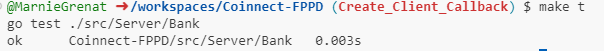
\includegraphics[width=1\linewidth]{assets/image.png}
    \caption{bank test output}
    \label{fig:enter-label}
\end{figure}
\end{document}